\documentclass[a4paper, 11pt]{article}

\usepackage[a4paper,margin=1in]{geometry}
\usepackage[french]{babel}
\usepackage[utf8]{inputenc}
\usepackage[T1]{fontenc}
\usepackage{lmodern}
\usepackage{listings}
\usepackage{graphicx}
\usepackage{amsmath}
\usepackage{framed}
\usepackage{amsfonts}
\usepackage{caption}
\usepackage{subcaption}
\usepackage{listings}
\usepackage{tabularx}
\usepackage{color}
\usepackage[dvipsnames]{xcolor}
\usepackage{fancyhdr}
\usepackage{lastpage}
\usepackage{tikz}

\usetikzlibrary{matrix}



\graphicspath{{../imgs/}}


\definecolor{morange}{RGB}{237,106,90}
\definecolor{mgreen}{RGB}{63,127,95}
\definecolor{mpurple}{RGB}{127,0,85}

\lstset{
  basicstyle=\small\ttfamily, % Global Code Style
  captionpos=b, % Position of the Caption (t for top, b for bottom)
  extendedchars=true, % Allows 256 instead of 128 ASCII characters
  tabsize=2, % number of spaces indented when discovering a tab
  columns=fixed, % make all characters equal width
  keepspaces=true, % does not ignore spaces to fit width, convert tabs to spaces
  showstringspaces=false, % lets spaces in strings appear as real spaces
  breaklines=true, % wrap lines if they don't fit
  frame=trbl, % draw a frame at the top, right, left and bottom of the listing
  frameround=tttt, % make the frame round at all four corners
  framesep=4pt, % quarter circle size of the round corners
  numbers=left, % show line numbers at the left
  numberstyle=\tiny\ttfamily, % style of the line numbers
  commentstyle=\color{mgreen}, % style of comments
  keywordstyle=\color{mpurple}, % style of keywords
  stringstyle=\color{morange}, % style of strings
}

% TAILLE DES PAGES (A4 serré)

\setlength{\parindent}{0pt}
\setlength{\parskip}{1em}
%% \setlength{\textwidth}{17cm}
%% \setlength{\textheight}{24cm}
%% \setlength{\oddsidemargin}{-.7cm}
%% \setlength{\evensidemargin}{-.7cm}
%% \setlength{\topmargin}{-.5in}


\pagestyle{fancy}
\renewcommand{\headrulewidth}{0pt}
\renewcommand{\footrulewidth}{0.6pt}% default is 0pt
\lhead{}
\rhead{}
\lfoot{Page \thepage\ of \pageref{LastPage}}
\rfoot{Rémi Lespinet}
\cfoot{}
\cfoot{}



\newcounter{cquestion}
\renewcommand{\thecquestion}{\arabic{cquestion}}
\newenvironment{question}
{\par \vspace{0.5em} \noindent \stepcounter{cquestion} \hspace{-1em}
 $\bullet$ \underline{Q\thecquestion :}}
{}

\newenvironment{note}
{\begin{framed} \textbf{Note : }}
{\end{framed}}


% Commandes de mise en page
\newcommand{\file}[1]{\lstinline{#1}}
\newcommand{\name}[1]{\emph{#1}}
\newcommand{\Fig}[1]{Fig \ref{#1} p. \pageref{#1}}
\newcommand{\Figure}[1]{Figure \ref{#1} p. \pageref{#1}}
\newcommand{\Tab}[1]{Tab \ref{#1} p. \pageref{#1}}
\newcommand{\Table}[1]{Table \ref{#1} p. \pageref{#1}}
\newcommand{\itemi}{\item[$\bullet$]}
% Commandes color
\newcommand{\colgood}[1]{\color{ForestGreen} #1}
\newcommand{\colbad}[1]{\color{BrickRed} #1}


% Commandes de maths
\newcommand{\function}[3]{#1 : #2 \to #3}
\newcommand{\intn}[2]{\left\{ #1 \dots #2 \right\}}
\newcommand{\intr}[2]{\left[ #1 ; #2 \right]}
\newcommand{\intro}[2]{\left] #1 ; #2 \right[}
\newcommand{\dotp}[2]{\langle #1, #2 \rangle}
\newcommand{\logn}[1]{\ln\left( #1\right)}
%% \newcommand{\det}[1]{\left| #1 \right|}
\newcommand{\pd}[2]{\frac{\partial #1}{\partial #2}}
\newcommand{\norm}[1]{\|#1\|}
\newcommand{\set}[2]{\left\{ #1 \hspace{.5em} ; \hspace{.5em}#2 \right\}}
\newcommand{\tr}[1]{Tr\left( #1 \right)}
\newcommand{\pcond}[2]{p(#1 \hspace{-.2em}\mid\hspace{-.2em} #2)}


\newcommand{\iid}{i.i.d }
\newcommand{\wrt}{w.r.t }

% Commandes informatique
\newcommand{\pfun}[1]{{\textbf{\texttt{#1}}}}

\newcommand{\ipart}[1]{\vspace{0.5em}\textbf{#1}\vspace{0.5em}}



\pagenumbering{arabic}

\title{\textsc{Reinforcement learning - MVA 2017/2018 \\ \emph{Homework 1}} }
\author{Rémi Lespinet}
\date{}

\begin{document}

\maketitle
\thispagestyle{fancy}

% p(s0 | s0, a0) = 0.45
% p(s2 | s0, a0) = 0.55

% p(s2 | s0, a1) = 1.00

% ####

% p(s2 | s1, a0) = 1.00

% p(s0 | s1, a1) = 0.5
% p(s1 | s1, a1) = 0.4
% p(s2 | s1, a1) = 0.1

% ####

% p(s0 | s2, a0) = 0.6
% p(s2 | s2, a0) = 0.4

% p(s1 | s2, a1) = 0.9
% p(s2 | s2, a1) = 0.1

\section{Dynamic Programming}

\begin{question}
  The transition table and the reward table for the graph of the
  exercice are presented in tables \ref{tab:transition-table} and
  \ref{tab:reward-table} respectively

  \begin{table}[h!]
    \centering
    \begin{tabular}{|c|c|c|c||c|c|c|}
      \hline
      & \multicolumn{3}{c||}{\textbf{a0}} & \multicolumn{3}{c|}{\textbf{a1}}\\
      \hline
      & s0 & s1 & s2 & s0 & s1 & s2 \\
      \hline
      s0 & 0.45 & 0.00 & 0.55 & 0.00 & 0.00 & 1.00 \\
      s1 & 0.00 & 0.00 & 1.00 & 0.50 & 0.40 & 0.10 \\
      s2 & 0.60 & 0.00 & 0.40 & 0.00 & 0.90 & 0.10 \\
      \hline
    \end{tabular}
    \captionof{table}{Representation of the transition table
      corresponding to the graph} \label{tab:transition-table}
  \end{table}

  \begin{table}[h!]
    \centering
    \begin{tabular}{|c|c|c|}
      \hline
      & a0 & a1 \\
      \hline
      s0 & -0.40 & 0.00 \\
      s1 & 2.00 & 0.00 \\
      s2 & -1.00 & -0.50 \\
      \hline
    \end{tabular}
    \captionof{table}{Representation of the reward table corresponding
      to the graph} \label{tab:reward-table}
  \end{table}


  % \begin{table}[h!]
  %   \centering
  %   \begin{tabular}{|c|c|c|}
  %     \hline
  %     & a0 & a1 \\
  %     \hline
  %     s0 & \begin{tabular}{c}
  %            $\pcond{s0}{s0, a0} = 0.45$ \\
  %            $\pcond{s2}{s0, a0} = 0.55$
  %          \end{tabular}
  %     & $\pcond{s2}{s0, a1} = 1.00$ \\
  %     \hline
  %     s1 & $\pcond{s2}{s1, a0} = 1.00$
  %          & \begin{tabular}{l}
  %              $\pcond{s0}{s1, a1} = 0.5$ \\
  %              $\pcond{s1}{s1, a1} = 0.4$ \\
  %              $\pcond{s2}{s1, a1} = 0.1$ \\
  %            \end{tabular}
  %     \\
  %     \hline
  %     s2 & \begin{tabular}{l}
  %            $\pcond{s0}{s2, a0} = 0.6$ \\
  %            $\pcond{s2}{s2, a0} = 0.4$ \\
  %          \end{tabular}
  %     &
  %       \begin{tabular}{l}
  %         $\pcond{s1}{s2, a1} = 0.9$ \\
  %         $\pcond{s2}{s2, a1} = 0.1$ \\
  %       \end{tabular}
  %     \\
  %     \hline
  %   \end{tabular}
  %   \captionof{table}{Representation of the transition table corresponding to the graph
  %     start for $K=4$ } \label{tab:table}
  % \end{table}

  % \begin{table}[h!]
  %   \centering
  %   \begin{tabular}{|c|c|c|c|}
  %     \hline
  %     & s0 & s1 & s2 \\
  %     \hline
  %     s0
  %     & \begin{tabularx}{0.2\textwidth}{X|X}
  %         \textbf{0.45} & 0.00
  %       \end{tabularx} & \begin{tabularx}{0.2\textwidth}{X|X}
  %                         0.00 & 0.00
  %                       \end{tabularx} & \begin{tabularx}{0.2\textwidth}{X|X}
  %                                         \textbf{0.55} & \textbf{1.00}
  %                                       \end{tabularx} \\
  %     \hline
  %     s1
  %     & \begin{tabularx}{0.2\textwidth}{X|X}
  %         0.00 & \textbf{0.50}
  %       \end{tabularx} & \begin{tabularx}{0.2\textwidth}{X|X}
  %                         0.00 & \textbf{0.40}
  %                       \end{tabularx} & \begin{tabularx}{0.2\textwidth}{X|X}
  %                                         \textbf{1.00} & \textbf{0.10}
  %                                       \end{tabularx} \\
  %     \hline
  %     s2
  %     & \begin{tabularx}{0.2\textwidth}{X|X}
  %         \textbf{0.60} & 0.00
  %       \end{tabularx} & \begin{tabularx}{0.2\textwidth}{X|X}
  %                         0.00 & \textbf{0.90}
  %                       \end{tabularx} & \begin{tabularx}{0.2\textwidth}{X|X}
  %                                         \textbf{0.40} & \textbf{0.10}
  %                                       \end{tabularx} \\
  %     \hline
  %   \end{tabular}
  %   \captionof{table}{Representation of the transition table corresponding to the graph
  %     start for $K=4$ } \label{tab:table}
  % \end{table}


  % TODO select table

\end{question}

\begin{question}
  The Policy evaluation and Value iteration algorithm are implemented
  in the file \file{lib_tp1_ex1.py}. The figure
  \ref{fig:VI-convergence} represents the distance to the optimal
  value $\norm{v^k - v^*}$ as a function of the number of iteration
  $k$.

  For the Policy evaluation, We have
  \begin{equation*}
    V^\pi(x) = r(x, \pi(x)) + \gamma \sum_y { \pcond{y}{x, \pi(x)} } V^\pi(y)
  \end{equation*}
  Which written in matrix form gives
  \begin{equation*}
    V^\pi = R^{\pi} + \gamma P^{\pi} V^\pi
  \end{equation*}
  With
  \begin{equation*}
    P^{\pi} =
    \begin{tikzpicture}[baseline=(current bounding box.center),
      large/.style={font=\large}]
      \matrix (M)[matrix of math nodes, nodes in empty cells,
      left delimiter={[}, right delimiter={]},
      column sep={3.2em,between origins},
      row sep={1.2em,between origins}
      ]{
        \pcond{x_1}{x_1, \pi(x_1)} &  & \hdots &  & \pcond{x_N}{x_1, \pi(x_1)} \\
        & & & & \\
        \vdots & & & & \vdots \\
        & & & & \\
        \pcond{x_1}{x_N, \pi(x_N)} &  & \hdots &  & \pcond{x_N}{x_N, \pi(x_N)} \\
      };
      % \draw(M-1-4.north)--(M-9-4.south);
      % \draw(M-4-1.west)--(M-4-9.east);
      % \node[large] at (M-2-7){$0$};
      % \node[large] at (M-7-2){$0$};
      % \node[large] at (M-7-7){$0$};
    \end{tikzpicture}
  \end{equation*}
  Hence
  \begin{equation*}
    (I - \gamma P^{\pi}) V^\pi = R^\pi
  \end{equation*}
  If we have $|X|$ states and $|A|$ actions, the complexity of
  evaluating a policy by this method is the cost of inverting a linear
  system $O(|X|^3)$ (the cost of evaluating $P^{\pi}$ and $R^\pi$ are
  negligeable, in fact we could directly do the calculation directly
  without calculating them).  We could also compute it iteratively
  using Bellman equations, which would lead to the number of
  iterations $K$ times the cost of multiplying a $N \times N$ matrix
  by a $N$ vector, which would be $O \left( |X|^2 K \right)$ with
  $K = \dfrac{\log{r_{max} / \epsilon}}{\log{1/\gamma}}$.

  \begin{figure}[h]
    \centering
    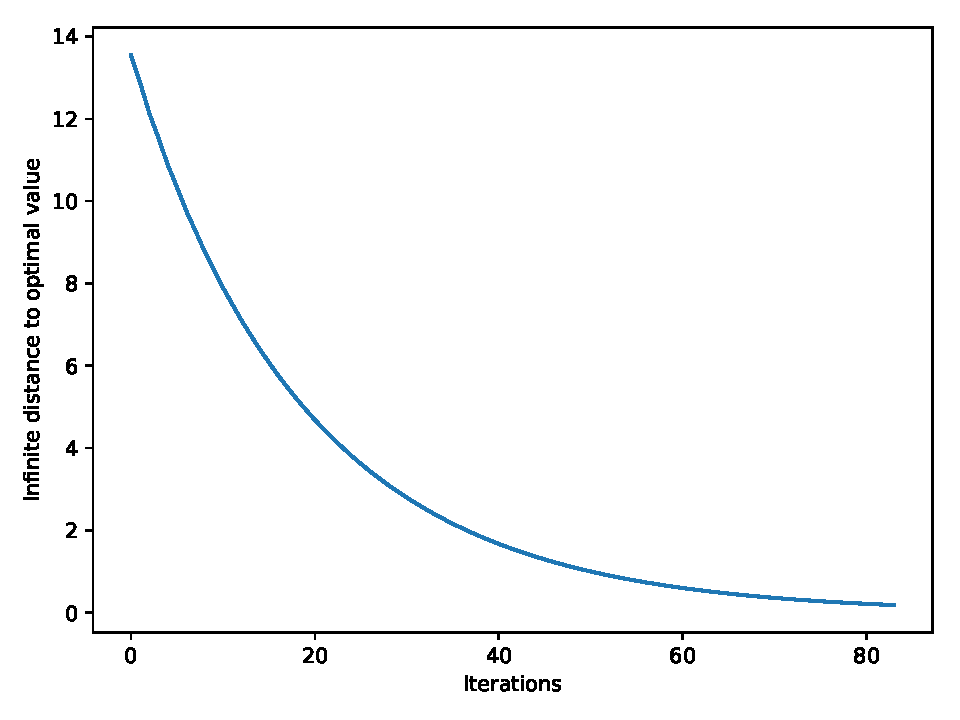
\includegraphics[width=0.7\textwidth]{VI_convergence}
    \caption{Convergence of the value iteration algorithm}\label{fig:VI-convergence}
  \end{figure}

\end{question}

\begin{question}
  The Policy Iteration (PI) algorithm is implemented in the file
  \file{lib_tp1_ex1.py}. In this case, the algorithm converges in
  $2$ iterations.

  At each iteration of the Policy Iteration algorithm, we need to
  compute a Policy evaluation, which has a cost of $O(|X|^3)$, and
  actually improve that policy, which has a cost of $O(|X|^2 |A|)$.

  The cost of the Value Iteration algorithm is $K$ (number of
  iterations) times the cost of computing
  \begin{equation*}
    V^{k+1}(x) = \max_a{r(x, a) + \gamma \sum_y { \pcond{y}{x, a} } V^{k}(y)}
  \end{equation*}
  which is $O(|X|^2 |A|)$

  Hence the costs are
  \begin{itemize}
  \item Value iteration : $O(|X|^2 |A| \dfrac{\log{\epsilon}}{\log{\gamma}})$
  \item Policy iteration (evaluation in close form): $O(L |X|^3)$
  \item Policy iteration (evaluation with Bellman equations): $O(L |X|^2 \dfrac{\log{\epsilon}}{\log{\gamma}})$
  \end{itemize}
  Where $L$ is the number of iteration of the most outer loop of the
  Policy iteration algorithm.

  We are doing mostly the same operations in the 2 algorithm, so the
  constants that stands before the big $O$ are almost the same.  Since
  here L is very small ($L=2$ in our case), and given the fact that we
  don't need a very precise evaluation at each step, using the
  iterative version of the policy evaluation with a relatively large
  $\epsilon$, should lead to a much lower constant, and hence a much
  faster convergence. In our case, because the number of states is
  small, solving the linear system is also very cheap which explains
  why the policy iteration is faster (In fact if it wouldn't, we would
  always use value iteration, which retrieves the policy for free, and
  policy iteration would be pointless).

\end{question}

\section{Reinforcement Learning}

\begin{question}

  \ipart{Policy Evaluation}

  First, we define the policy that goes right if possible, otherwise
  up. The figure \ref{fig:policy-right-or-up} represents the
  policy. (I only changed the colors so that we can see the missing
  cell, and a line in \file{gridrender.py} to export in postscript)

  \begin{figure}[h]
    \centering
    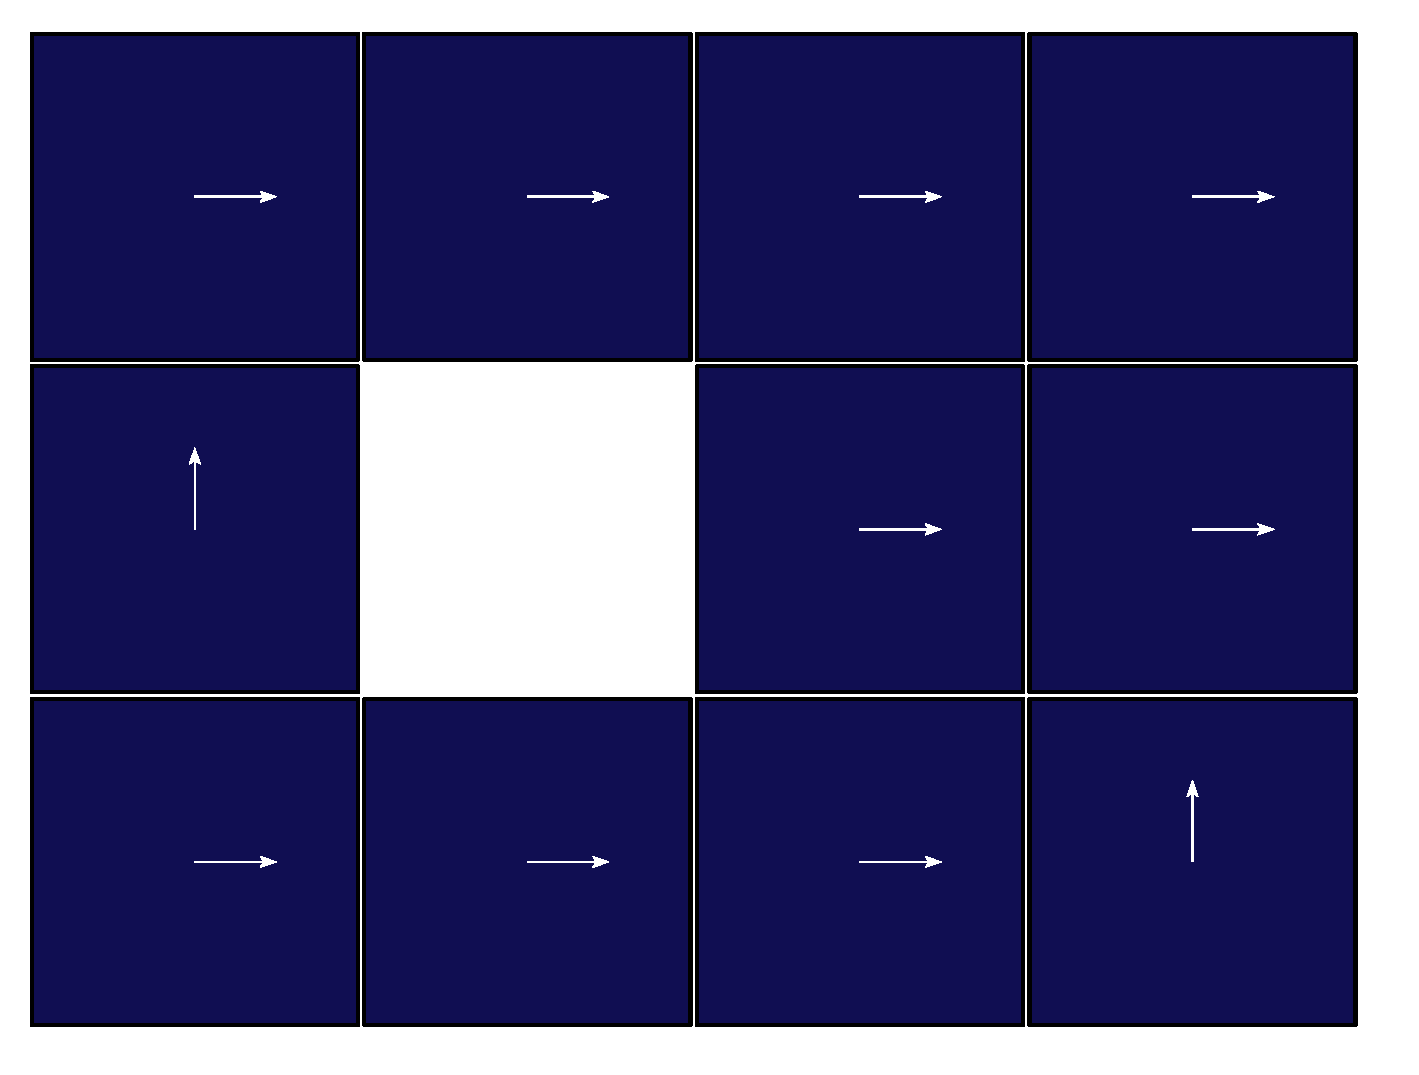
\includegraphics[width=0.7\textwidth]{policy_right_or_up}
    \caption{Representation of the policy to evaluate}\label{fig:policy-right-or-up}
  \end{figure}

  The estimated state value function obtained by a run of the
  Monte-Carlo algorithm (function \pfun{EvaluatePolicy} in the file
  \file{lib_tp1_ex1.py}) with $10000$ iterations is given of figure
  \ref{fig:q-policy} (to be compared with the real state value
  function for this policy given, given in figure \ref{fig:q-policy-ref}

  \begin{figure}[h]
    \centering
    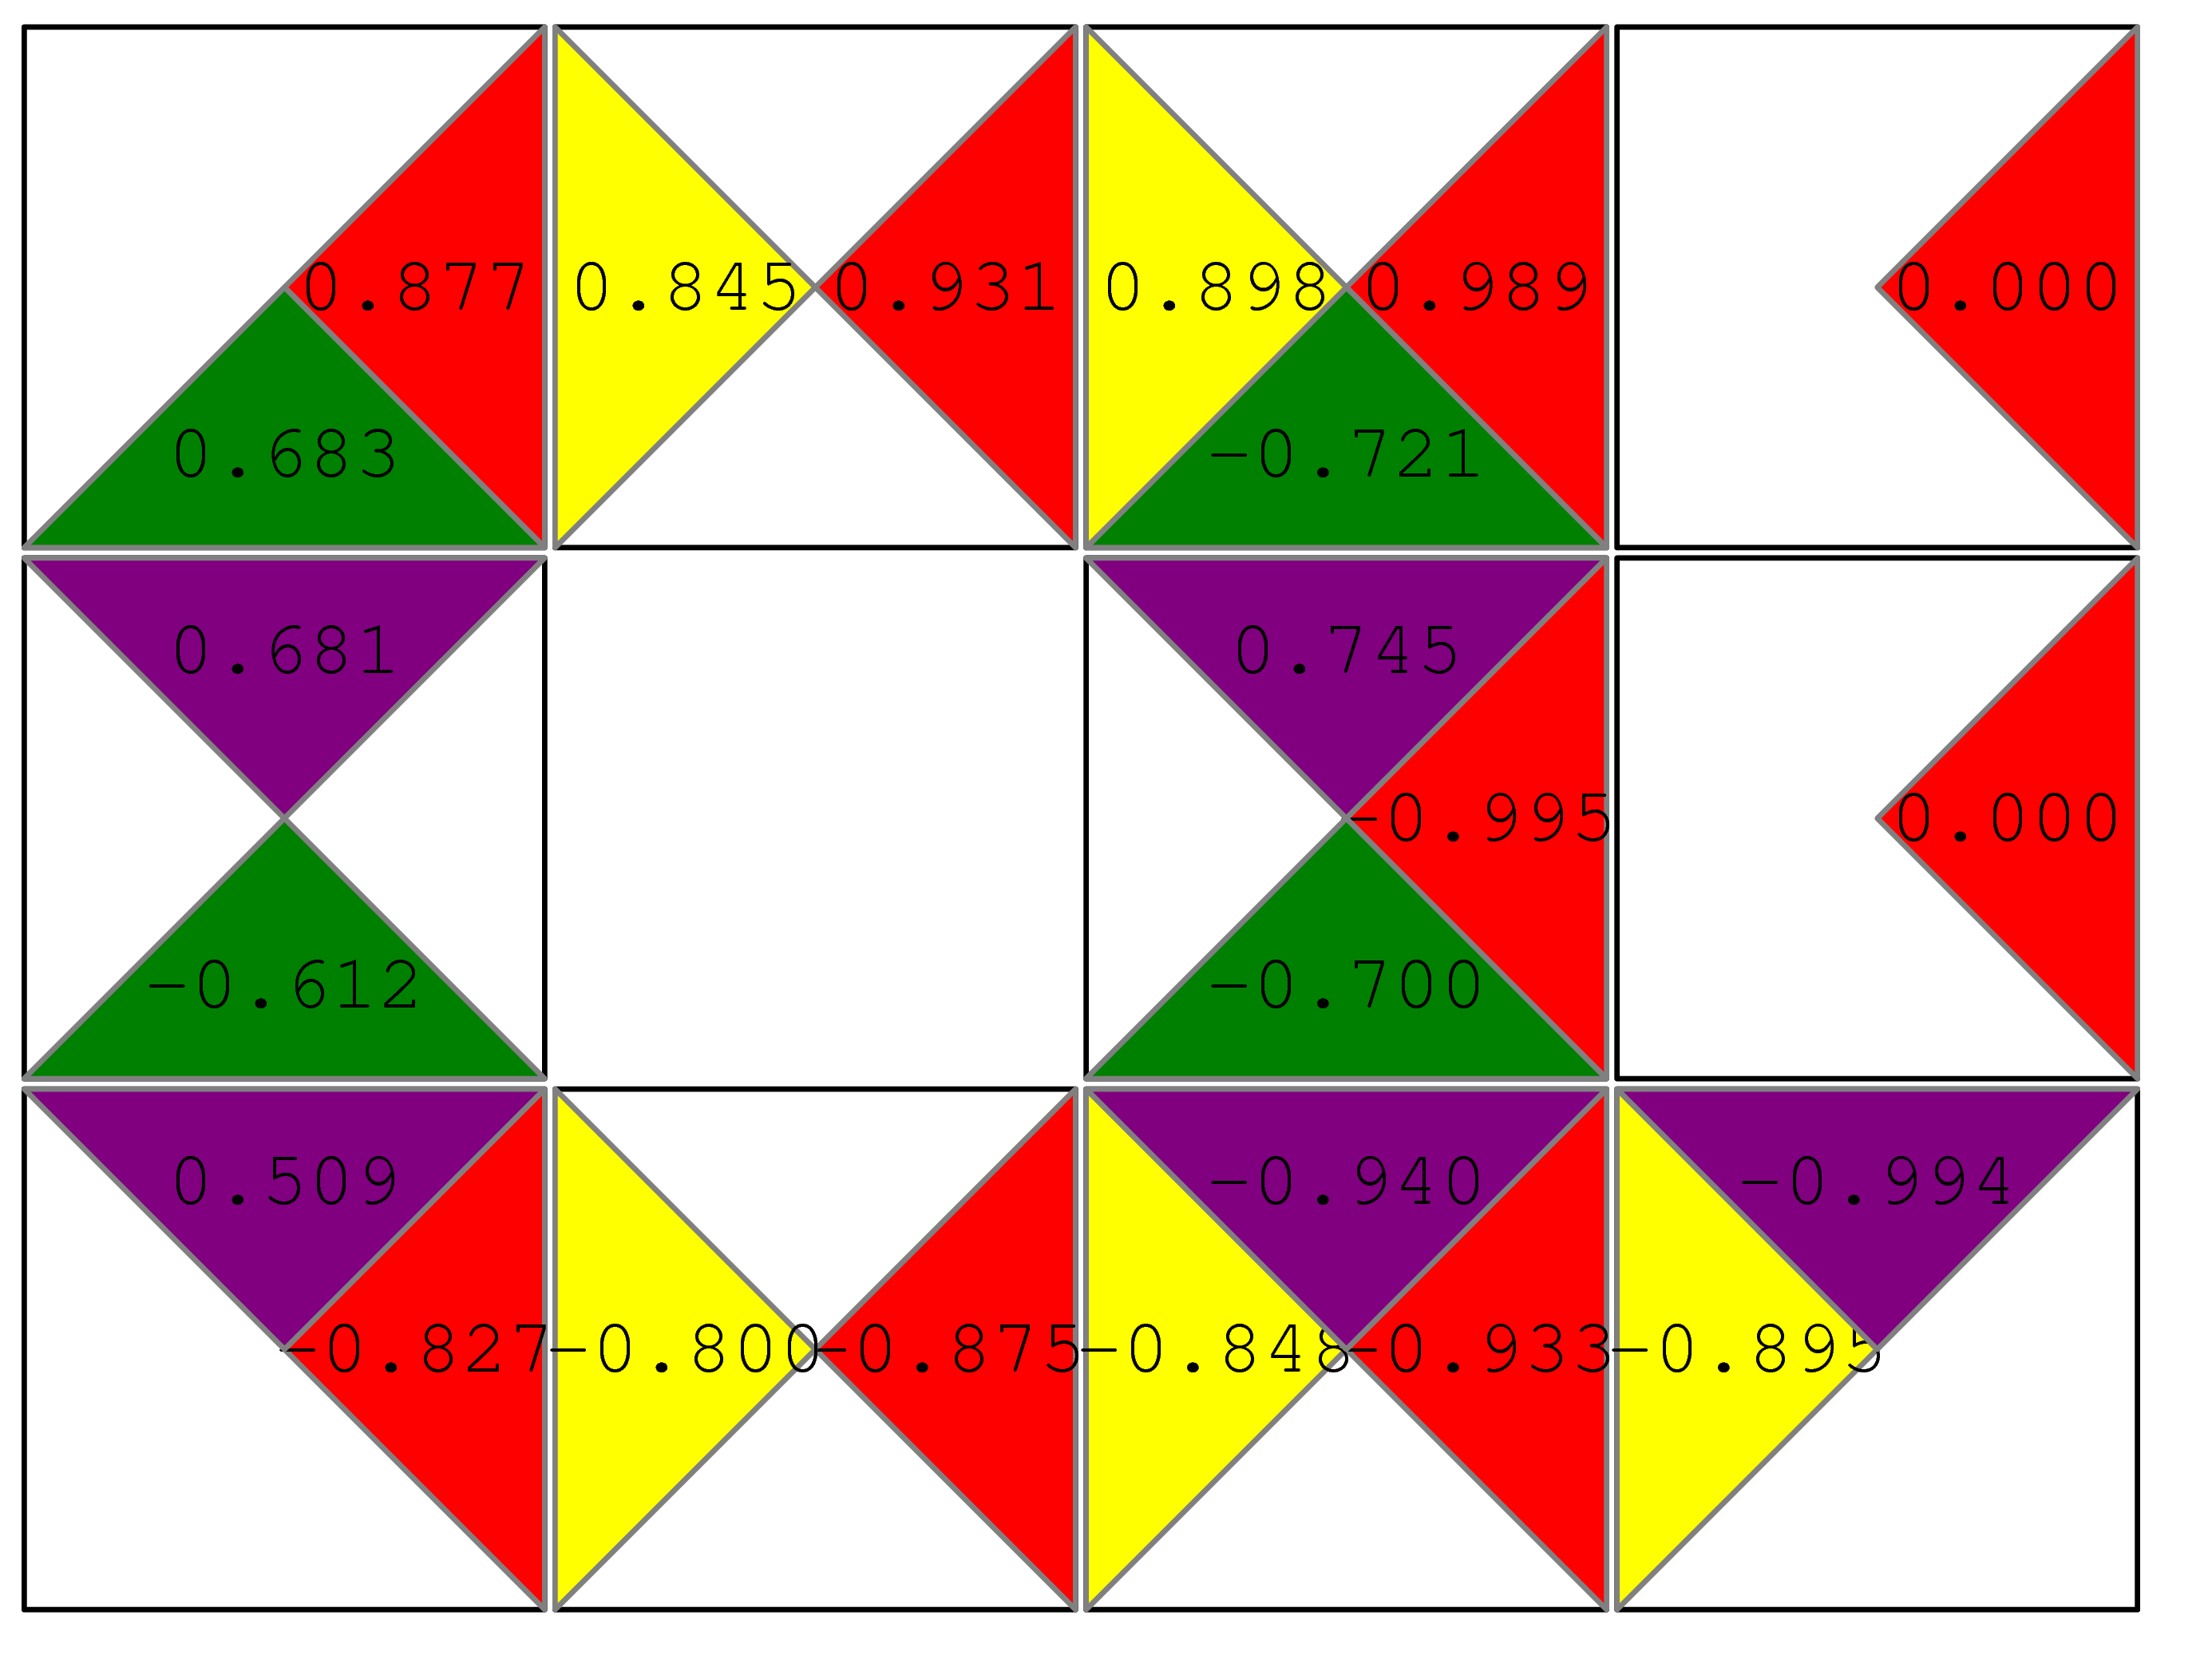
\includegraphics[width=0.8\textwidth]{q_policy}
    \caption{Representation of the state value $\hat{Q}^\pi$ function obtained when
      evaluating the policy with the Monte-Carlo algorithm ($10000$
      iterations)}\label{fig:q-policy}
  \end{figure}

  \begin{figure}[h]
    \centering
    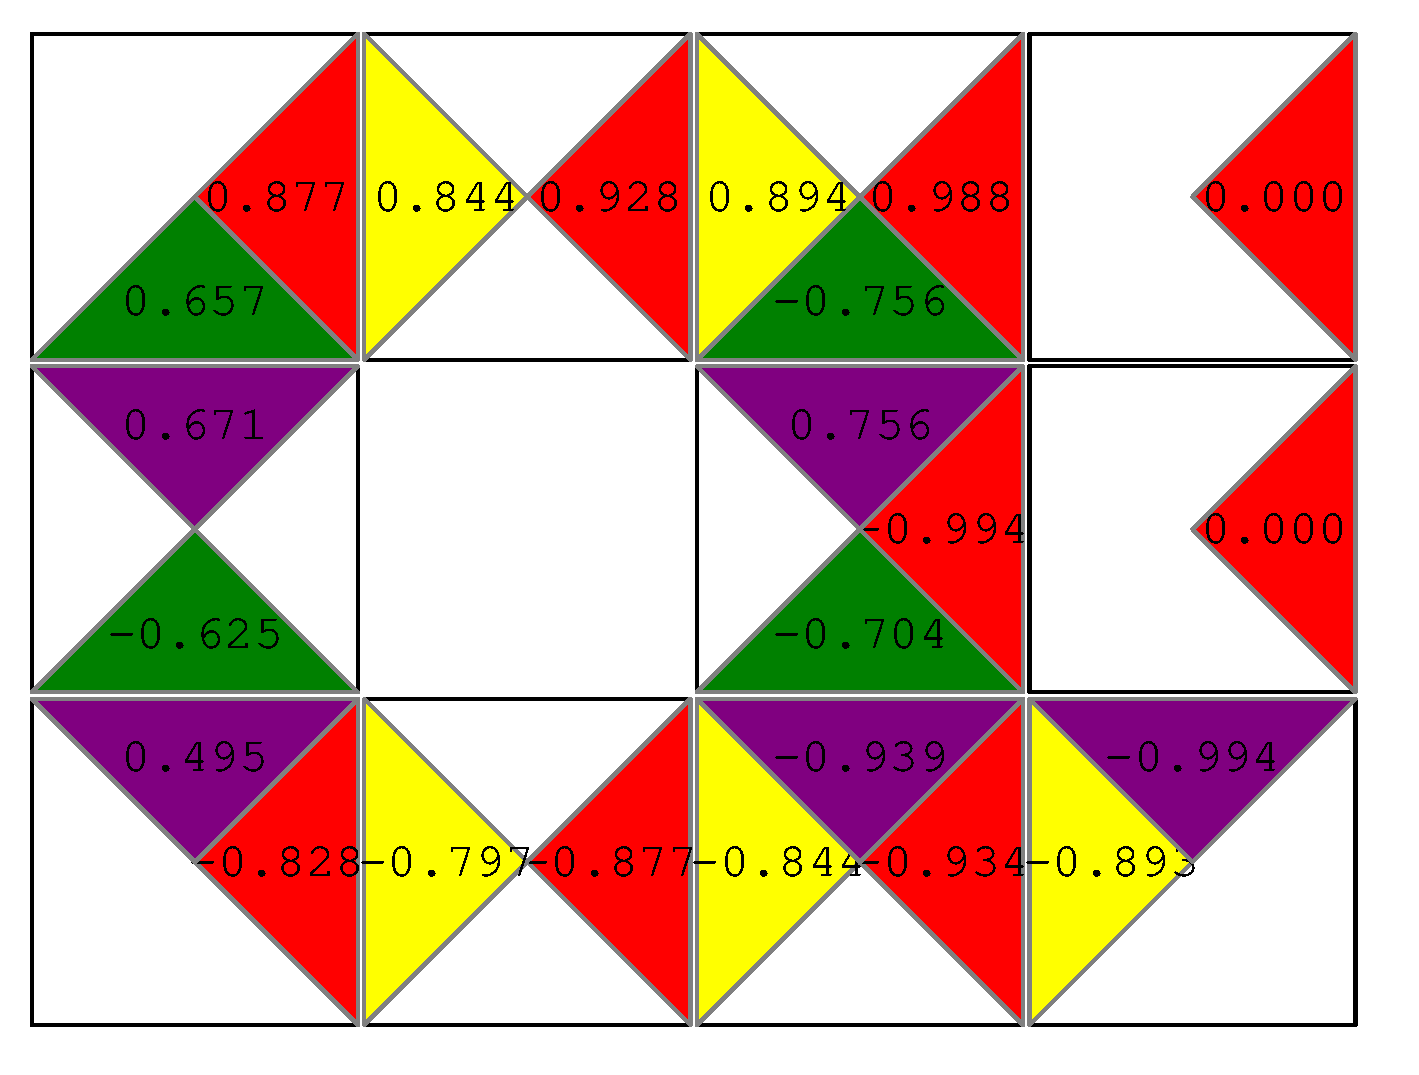
\includegraphics[width=0.8\textwidth]{q_policy_ref}
    \caption{Representation of the real state value function
      $Q^\pi$ given}\label{fig:q-policy-ref}
  \end{figure}

  \clearpage
  The results are good, since $x_3$ (in row $0$ and column $3$) is the
  good state (reward $+1$) and $x_6$ (in row $1$ and column $3$) is
  the bad state (reward $-1$). From the policy, we go right if we can,
  so basically, we need to be in one of the green cells (in figure
  \ref{fig:q-policy-explained}) after step 1 if we want a positive reward,
  and that's exactly what we get when looking at the representation of
  Q.

  \begin{figure}[h]
    \centering
    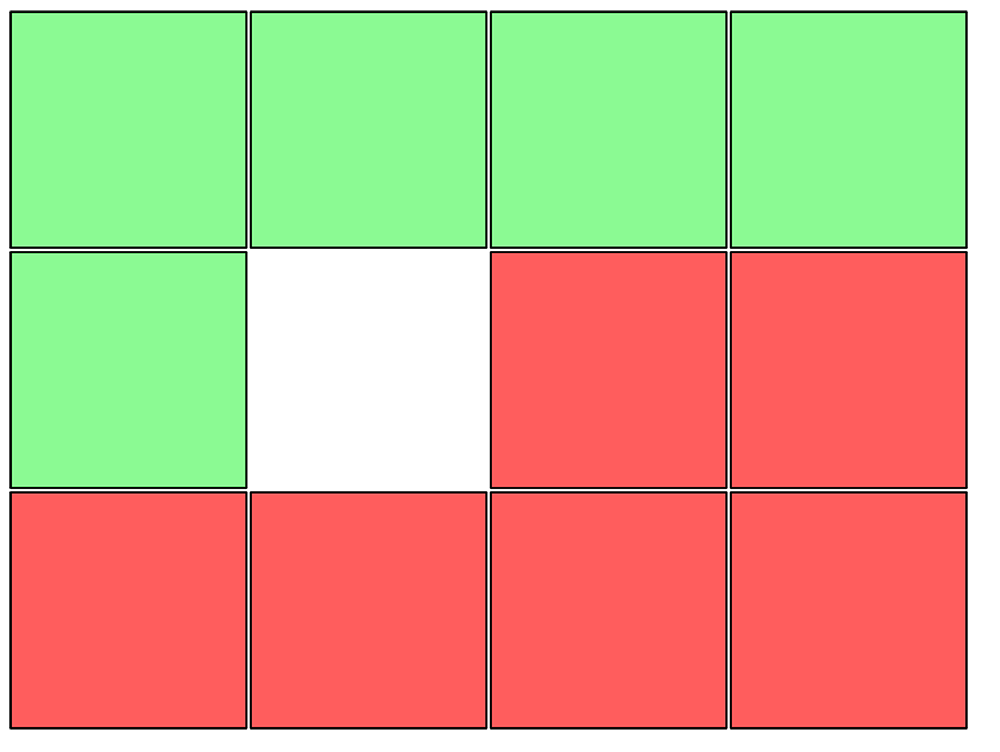
\includegraphics[width=0.5\textwidth]{q_policy_explained}
    \caption{Green cells (resp. red cells) represent the cells we have
      to be after the first step to obtain a positive (resp. negative)
      reward (for the policy)}\label{fig:q-policy-explained}
  \end{figure}

  The figure \ref{fig:j-100000} represents the evolution of $J_k - J^\pi$
  as a function of the number of iteration $k$

  \begin{figure}[h]
    \centering
    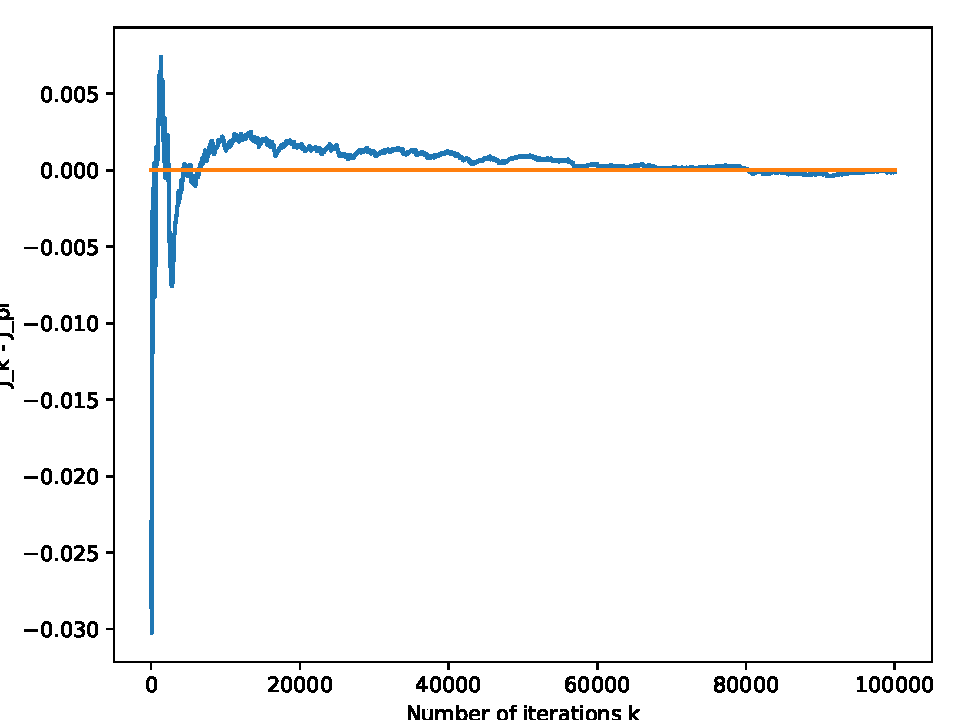
\includegraphics[width=0.7\textwidth]{j_100000}
    \caption{Evolution of $J_k - J^\pi$ as a function of the number of
      iteration $k$}\label{fig:j-100000}
  \end{figure}

  We can see that we have a good estimate of $V^\pi$ really fast.
  In our example, there is a $10\%$ probability of going the
  other direction when we do a step (by looking at the source code),
  this introduces a random in our simulation (if we had $100\%$
  probability of going in the direction we want, we would have
  basically estimated $Q^\pi$ as soon as we would have tried
  all the pairs (state, action)).

  \ipart{Policy optimization}

  The Q-learning algorithm is implemented in the file
  \file{lib_tp1_ex1.py}.

\end{question}

\begin{question}
  I've defined the step size to be the number of time we went through
  the same (state, action) Thus it satisfies the stochastic
  requirements.
  \begin{equation*}
    \alpha_i(x, a) = \dfrac{1}{N_i(x, a)}
  \end{equation*}

  I've plotted $\norm{V_k - V^*}_{\infty}$ as a function of the number
  of iteration $k$ and the values of the reward cumulated over the
  episodes for different values of $\epsilon$, the results are
  presented in figure \ref{fig:comp-eps-5000} and \ref{fig:cum-rewards-200}

  \begin{figure}[h]
    \centering
    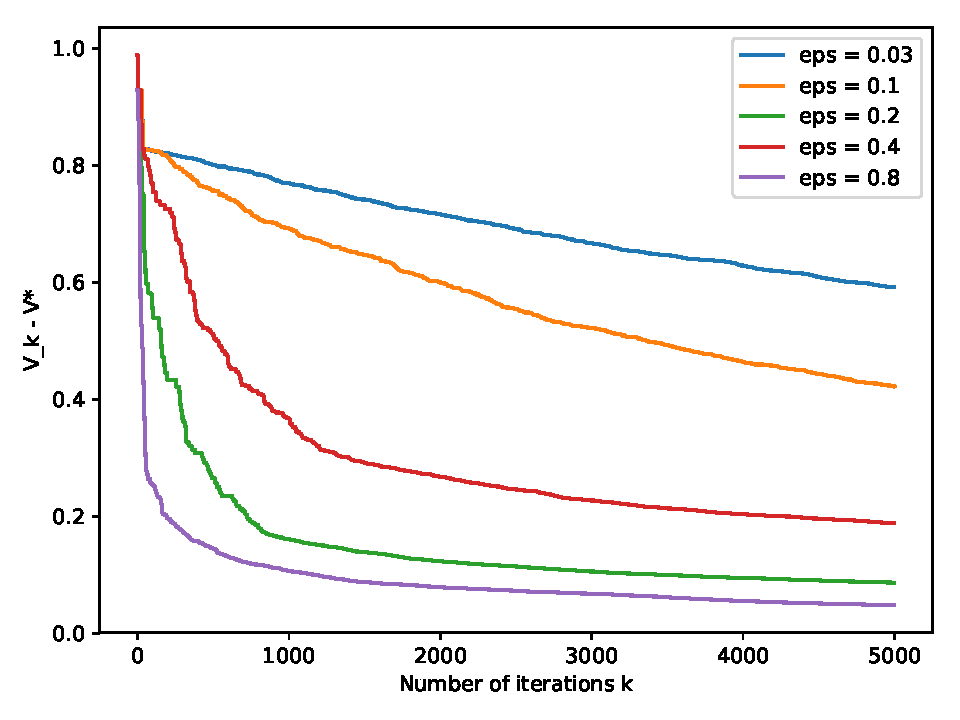
\includegraphics[width=0.7\textwidth]{comp_eps_5000}
    \caption{Evolution of $\norm{V_k - V^*}_{\infty}$ as a function of
      the number of iteration $k$ for different values of
      $\epsilon$}\label{fig:comp-eps-5000}
  \end{figure}

  We can see that if we take a large $\epsilon$, which means we are
  mainly exploring, the value decreases really fast compared to
  others, so this is a good strategy to have an accurate estimate of
  the statee value function, as expected. % In the figure \ref{fig:comp-eps-5000}, we
  % see that the curve for $\epsilon = 0.2$ and $\epsilon = 0.4$ goes
  % below the curve for $\epsilon = 0.8$ as the number of iteration
  % increases.

  The figure \ref{fig:cum-rewards-200} shows the evolution of the
  reward cumulated over episodes when the number of episodes is low.
  We see that the curve with $\epsilon = 0.03$ achieves the worst
  performance when the number of iteration is low, which correspond to
  the time where it does not know anything. The algorithm will learn
  very slowly, but will then exploit its knowledge to get the highest
  possible reward (see \ref{fig:cum-rewards-20000})

  \begin{figure}[h]
    \centering
    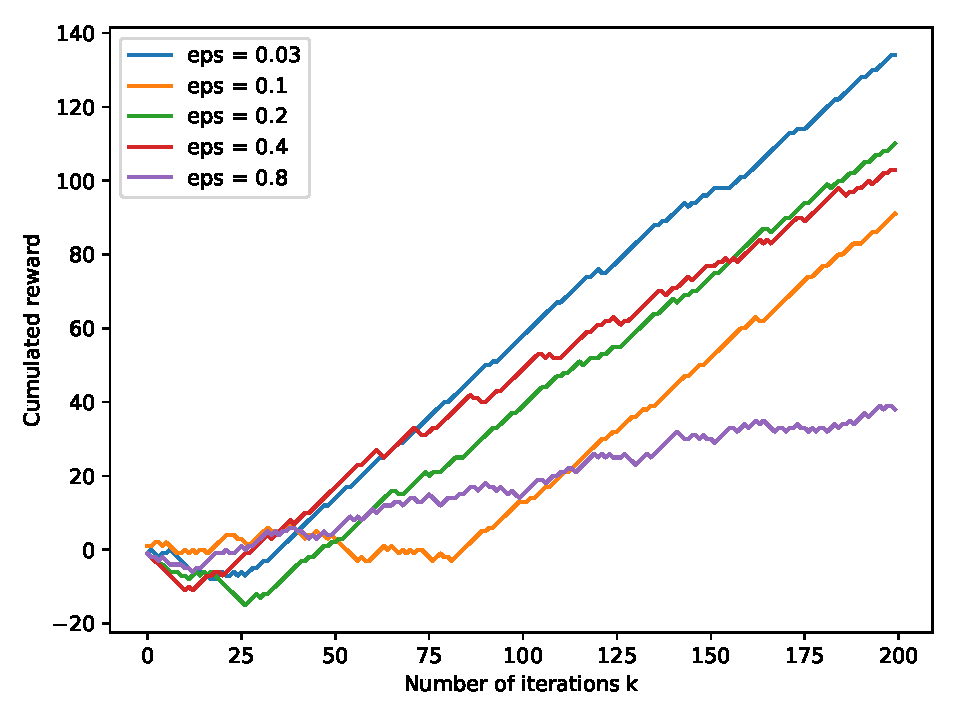
\includegraphics[width=0.7\textwidth]{cum_rewards_200}
    \caption{Evolution of the reward cumulated over episodes as a
      function of the number of iteration $k$ for different values of
      $\epsilon$}\label{fig:cum-rewards-200}
  \end{figure}

  This illustrates the exploration/exploitation tradeoff,
  High values of epsilon will explore very much, and
  hence produce accurate values of the state value function,
  at the cost of having a poor reward, as opposed to low
  values of epsilon, which would produce a high reward without
  exploring the problem very much.

  \begin{figure}[h]
    \centering
    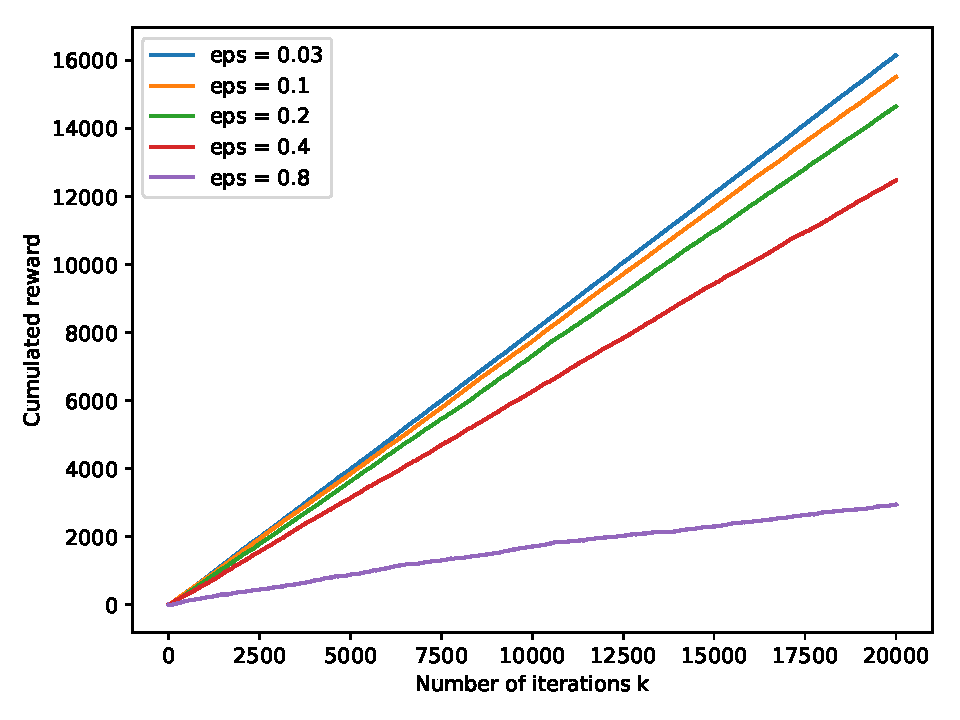
\includegraphics[width=0.7\textwidth]{cum_rewards_20000}
    \caption{Evolution of the reward cumulated over episodes as a
      function of the number of iteration $k$ for different values of
      $\epsilon$}\label{fig:cum-rewards-20000}
  \end{figure}

\end{question}

\clearpage
\begin{question}
  The initial distribution does not affect the optimal policy, because
  the optimal value achieves the highest value for all states.  The
  final policy for the grid problem is presented in figure
  \ref{fig:final-policy} In fact, we can verify it experimentally by
  changing the probability in the \pfun{reset} function.  For example
  with the code proposed below, which makes the nodes with the higher
  indices more probables, we obtain the same estimated optimal
  policy and estimated optimal value function.

  \begin{lstlisting}[language=Python]
    def reset(self):
        """
        Returns:
            An initial state randomly drawn from
            the initial distribution
        """
        states_prob = np.cumsum(np.arange(1, self.n_states + 1))
        p = np.random.randint(0, states_prob[-1])
        x_0 = np.argmax(states_prob > p)

        return x_0
  \end{lstlisting}


  \begin{figure}[h]
    \centering
    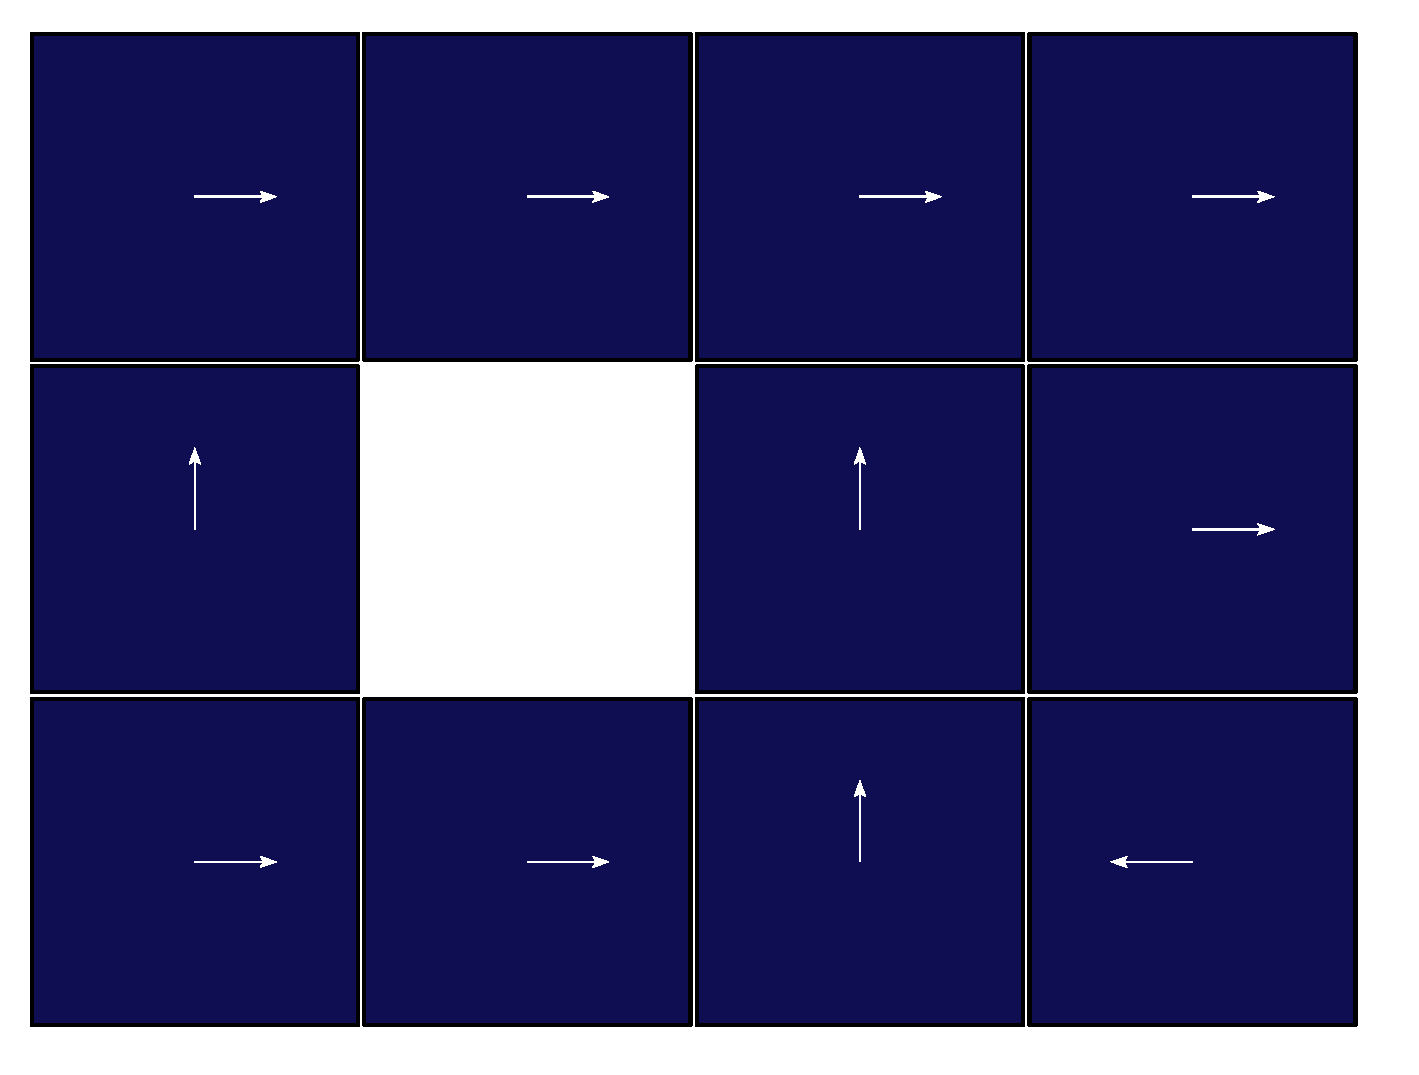
\includegraphics[width=0.7\textwidth]{final_policy}
    \caption{Estimated optimal policy obtained by an execution of the
      Q-learning algorithm with $\epsilon = 0.2$ and $N = 20000$
      episodes ($Tmax = 100$)}\label{fig:final-policy}
  \end{figure}


\end{question}

%% \begin{figure}[p]
%%   \centering
%%   \begin{subfigure}[t]{0.40\textwidth}
%%     \centering
%%     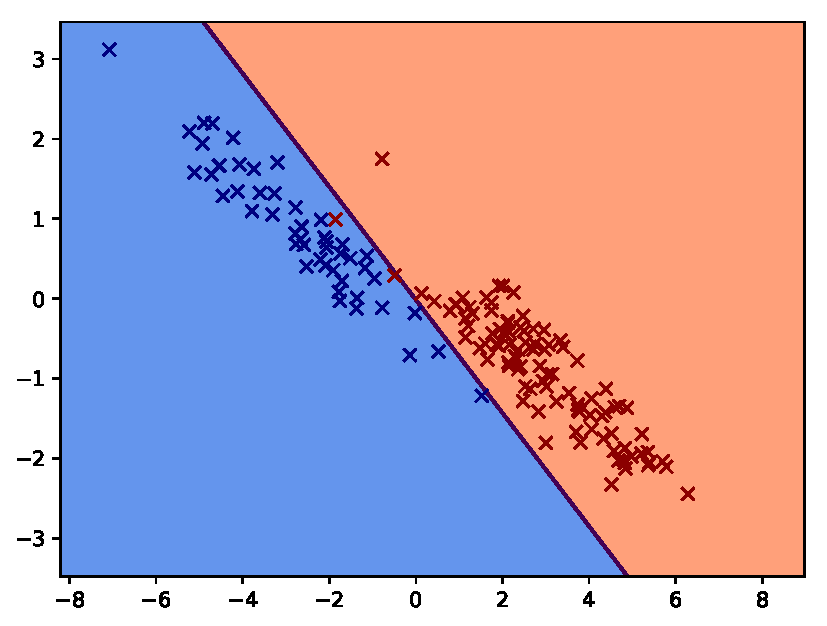
\includegraphics[width=\textwidth]{LDA_classificationA_train.pdf}
%%     \caption{Training observations A ($150$ points)}\label{fig:LDA-A-train}
%%   \end{subfigure}
%%   \quad
%%   \begin{subfigure}[t]{0.40\textwidth}
%%     \centering
%%     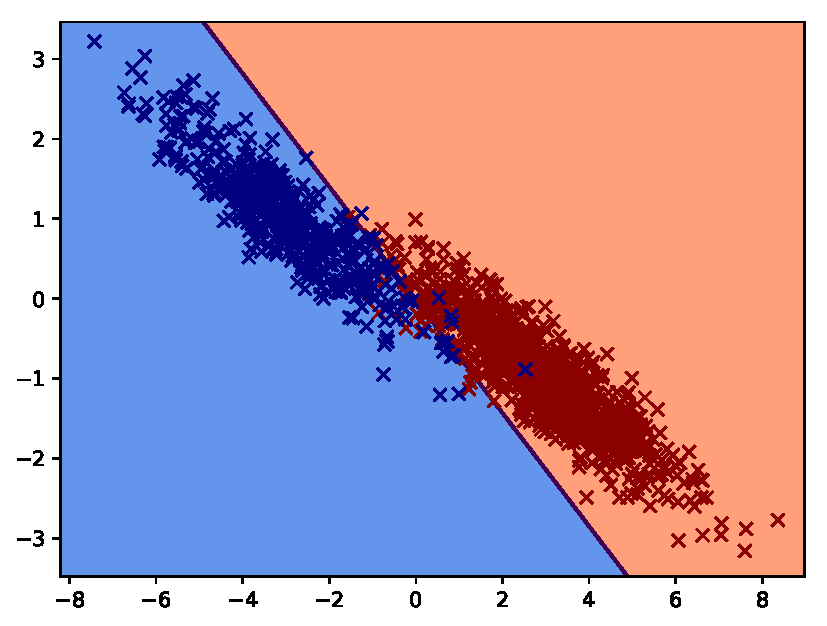
\includegraphics[width=\textwidth]{LDA_classificationA_test.pdf}
%%     \caption{Test observations A ($1500$ points)}\label{fig:LDA-A-test}
%%   \end{subfigure}
%%   \vskip\baselineskip
%%   \begin{subfigure}[t]{0.40\textwidth}
%%     \centering
%%     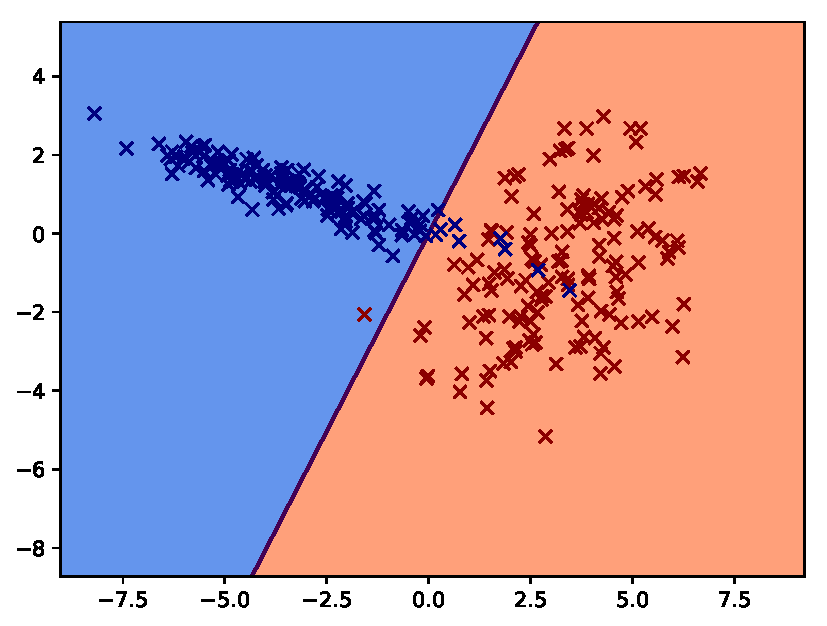
\includegraphics[width=\textwidth]{LDA_classificationB_train.pdf}
%%     \caption{Training observations B ($150$ points)}\label{fig:LDA-B-train}
%%   \end{subfigure}
%%   \quad
%%   \begin{subfigure}[t]{0.40\textwidth}
%%     \centering
%%     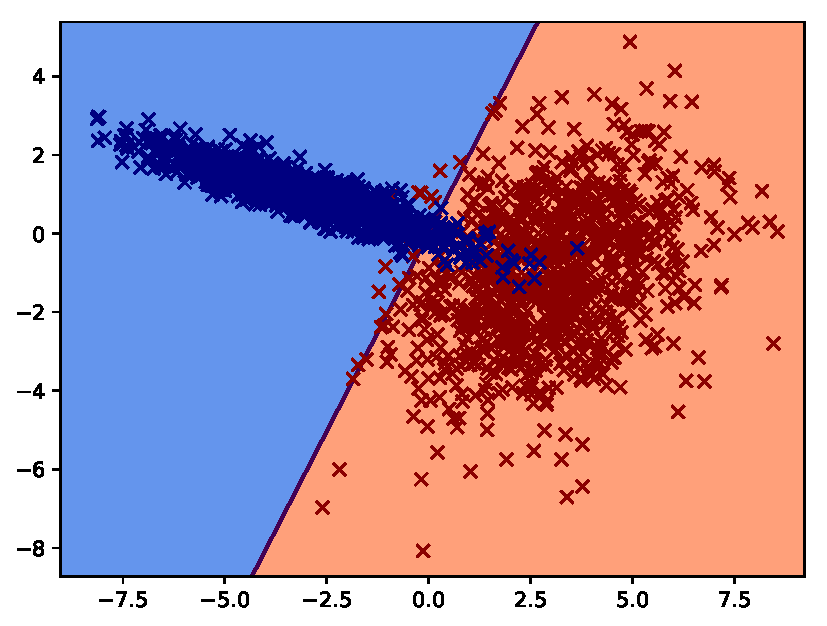
\includegraphics[width=\textwidth]{LDA_classificationB_test.pdf}
%%     \caption{Test observations B ($1500$ points)}\label{fig:LDA-B-test}
%%   \end{subfigure}
%%   \vskip\baselineskip
%%   \begin{subfigure}[t]{0.40\textwidth}
%%     \centering
%%     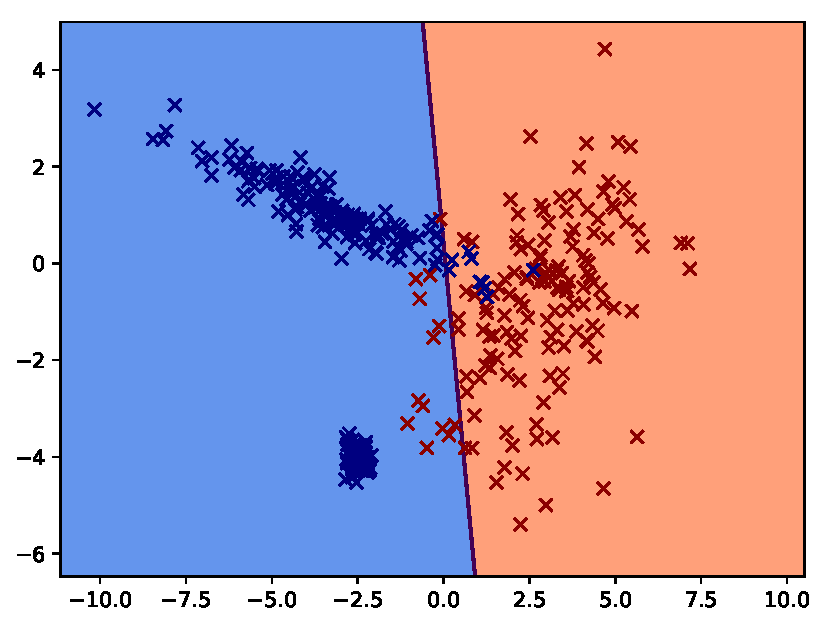
\includegraphics[width=\textwidth]{LDA_classificationC_train.pdf}
%%     \caption{Training observations C ($150$ points)}\label{fig:LDA-C-train}
%%   \end{subfigure}
%%   \quad
%%   \begin{subfigure}[t]{0.40\textwidth}
%%     \centering
%%     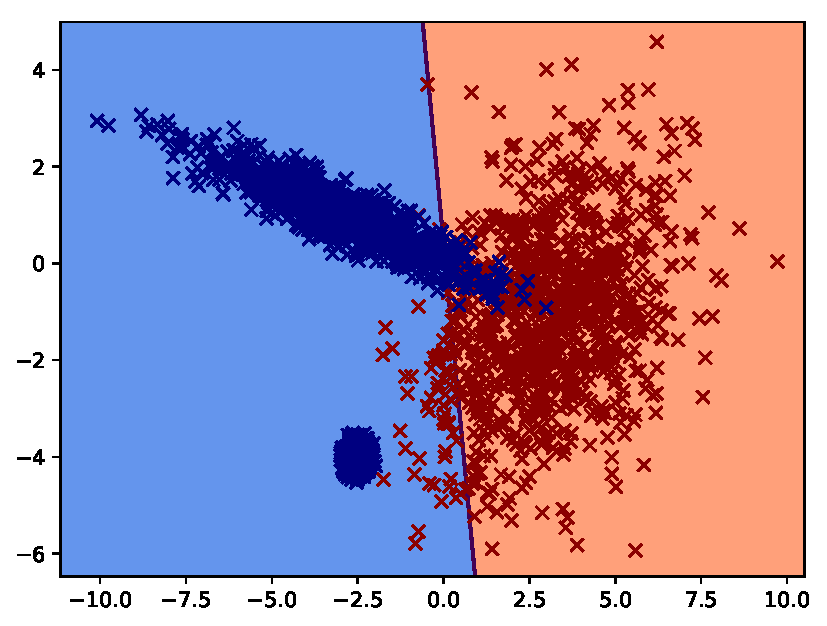
\includegraphics[width=\textwidth]{LDA_classificationC_test.pdf}
%%     \caption{Test observations C ($1500$ points)}\label{fig:LDA-C-test}
%%   \end{subfigure}
%%   \caption{Sample data and decision boundary representation for the LDA classifier on the three files}\label{fig:LDA}
%% \end{figure}


\end{document}
